\message{ !name(1.tex)}
\message{ !name(1.tex) !offset(512) }
\subsection{La genèse}
Comme expliqué au début de ce manuscrit, l'univers avant la recombinaison\footnote{Le moment où les électrons se lient aux protons pour former les premiers atomes.} est un plasma chaud et dense,
% composé des photons, des baryons, et de la matière noire. L'univers n'étant, initialemment, pas parfaitement homogène,
qui présente de faibles inhomogénéïtés.
% les surdensités présentes produisent des puits de potentiels,
Chaque surdensité produit un puit de potentiel,
dans lesquels les particules – les photons, les baryons, la matière noire – tombent.
Les photons et les baryons étant couplés, la pression de radiation augmente au fur et à mesure que la densité augmente. Se joue alors une compétition entre la gravité, qui tend à faire tomber les photons et les baryons dans les puits de potentiel, et la pression de radiation, qui tend à les repousser hors de ce puit de potentiel. Ainsi, les baryons et les photons tombent, puis rebondissent, puis retombent lorsque la pression de radiation devient trop faible, etc.
Ce processus crée donc des oscillations dans le plasma photon-baryon primordial. Comme dans tout milieu, ces oscillations donnent lieu à des ondes acoustiques, qui se propagent à la vitesse du son dans ce milieu. Celle-ci est définie comme
\begin{equation}
  \label{eq:sound_speed}
  c_{s} = \sqrt{\frac{1}{3(1 + R)}},
\end{equation}
où $R = \frac{3\rho_b}{4\rho_{\gamma}}$. Etant donné que la densité de photons $\rho_{\gamma}$ est bien supérieure à la densité de baryons $\rho_{b}$, la vitesse du son $c_s$ vaut $1/\sqrt{3}$ en bonne approximation. (\#prov en fait est-ce que c'est important de donner ca?)

\begin{figure}
  \centering
  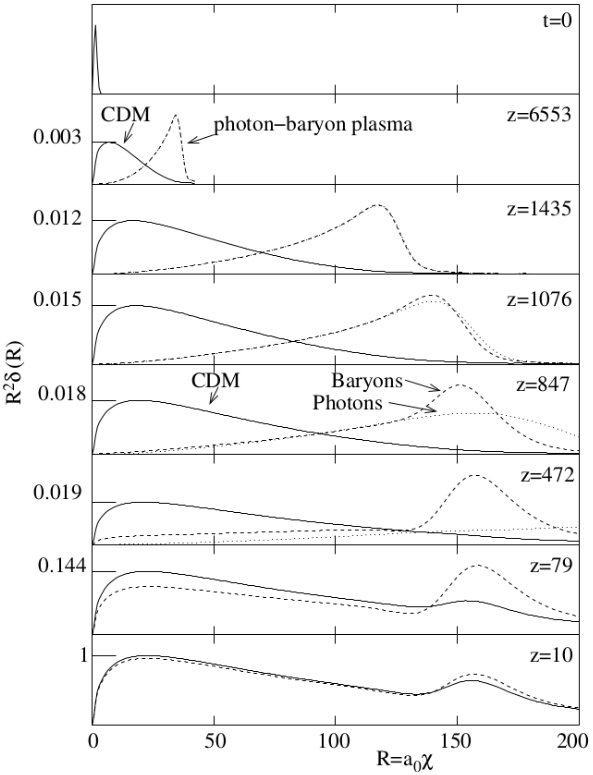
\includegraphics[scale=0.5]{bao_schema}
  \caption{bla}
  \label{fig:bao_schema}
\end{figure}
Ces ondes acoustiques se propagent donc dans le plasma primordial depuis chaque surdensité . La figure~\ref{fig:bao_schema} schématise le méchanisme pour une seule surdensité. A l'instant $t=0$, nous considérons donc une surdensité en $R = \SI{0}{\Mpc}$. Cette surdensité est composée de matière noire (CDM), de baryons et de photons. Le puis de potentiel créé fait s'effondrer les espèces présentes, jusqu'à ce que la pression de radiation devienne suffisante pour initier une onde acoustique. Au fur et à mesure que le temps s'écoule (le redshift diminue), le front d'onde dans le plasma photon-baryon se propage. Puis, à un redshift $z_{drag} \sim 1060$, les baryons se découplent des photons, et l'onde devient gelée. Ainsi la surdensité de baryon ne se propage plus, et les photons, qui n'interagissent plus avec les baryons, se propagent librement. La surdensité de matière noire à $R = \SI{0}{\Mpc}$, qui a continué de croître, tend à rappeler les baryons par effet gravitationnel. Cependant, la surdensité de baryon à $R \sim \SI{150}{\Mpc}$ produit aussi un puit de potentiel, dans lequel la matière noire alentour tombe progressivement. Ainsi, même si la majeure partie des baryons retombent dans le puit de potentiel créé par la surdensité initiale, un second puit de potentiel, formé par des baryons et de la matière noire, subsiste en $R \sim \SI{150}{\Mpc}$. Nous pouvons généraliser cette vue simplifier en une dimension à 3 dimensions : le front d'onde qui se propagent à partir de la surdensité initiale est alors sphérique, et le second puit de potentiel résultant est alors une sphère centrée sur la surdensité initiale et de rayon $R \sim \SI{150}{\Mpc}$. Cette distance d'environ $\SI{150}{\Mpc}$ est appelée \emph{horizon acoustique} : c'est la distance que l'onde sonore a pu parcourir avant d'être gelée. L'horizon acoustique est défini comme
\begin{equation}
  \label{eq:sound_horizon}
  r_\mathrm{d} = \int^{\infty}_{z_{drag}} \frac{c_{s}}{H(z)} dz ,
\end{equation}
et vaut $r_\mathrm{d} = \SI{147.18(29)}{\Mpc}$ selon~\ref{CITE planck2018}.

Ce processus a laissé des traces dans la distribution de matière à grande échelle : à chaque surdensité primordiale est associée une sphère de surdensité de rayon comobile $\SI{150}{\Mpc}$. Ainsi, lorsque nous observons aujourd'hui un traceur de la densité de matière, telle une galaxie, il est davantage probable d'en trouver d'autres, séparés du premier d'une distance comobile d'environ $\SI{150}{\Mpc}$. C'est ce que traduit le pic BAO présent dans la fonction de corrélation de la matière, montrée sur la figure~\ref{fig:CITE figure CF}


\message{ !name(1.tex) !offset(-34) }
